%% template.tex
%% from
%% bare_conf.tex
%% V1.4b
%% 2015/08/26
%% by Michael Shell
%% See:
%% http://www.michaelshell.org/
%% for current contact information.
%%
%% This is a skeleton file demonstrating the use of IEEEtran.cls
%% (requires IEEEtran.cls version 1.8b or later) with an IEEE
%% conference paper.
%%
%% Support sites:
%% http://www.michaelshell.org/tex/ieeetran/
%% http://www.ctan.org/pkg/ieeetran
%% and
%% http://www.ieee.org/

%%*************************************************************************
%% Legal Notice:
%% This code is offered as-is without any warranty either expressed or
%% implied; without even the implied warranty of MERCHANTABILITY or
%% FITNESS FOR A PARTICULAR PURPOSE!
%% User assumes all risk.
%% In no event shall the IEEE or any contributor to this code be liable for
%% any damages or losses, including, but not limited to, incidental,
%% consequential, or any other damages, resulting from the use or misuse
%% of any information contained here.
%%
%% All comments are the opinions of their respective authors and are not
%% necessarily endorsed by the IEEE.
%%
%% This work is distributed under the LaTeX Project Public License (LPPL)
%% ( http://www.latex-project.org/ ) version 1.3, and may be freely used,
%% distributed and modified. A copy of the LPPL, version 1.3, is included
%% in the base LaTeX documentation of all distributions of LaTeX released
%% 2003/12/01 or later.
%% Retain all contribution notices and credits.
%% ** Modified files should be clearly indicated as such, including  **
%% ** renaming them and changing author support contact information. **
%%*************************************************************************


% *** Authors should verify (and, if needed, correct) their LaTeX system  ***
% *** with the testflow diagnostic prior to trusting their LaTeX platform ***
% *** with production work. The IEEE's font choices and paper sizes can   ***
% *** trigger bugs that do not appear when using other class files.       ***                          ***
% The testflow support page is at:
% http://www.michaelshell.org/tex/testflow/

\documentclass[conference,final,]{IEEEtran}
% Some Computer Society conferences also require the compsoc mode option,
% but others use the standard conference format.
%
% If IEEEtran.cls has not been installed into the LaTeX system files,
% manually specify the path to it like:
% \documentclass[conference]{../sty/IEEEtran}





% Some very useful LaTeX packages include:
% (uncomment the ones you want to load)


% *** MISC UTILITY PACKAGES ***
%
%\usepackage{ifpdf}
% Heiko Oberdiek's ifpdf.sty is very useful if you need conditional
% compilation based on whether the output is pdf or dvi.
% usage:
% \ifpdf
%   % pdf code
% \else
%   % dvi code
% \fi
% The latest version of ifpdf.sty can be obtained from:
% http://www.ctan.org/pkg/ifpdf
% Also, note that IEEEtran.cls V1.7 and later provides a builtin
% \ifCLASSINFOpdf conditional that works the same way.
% When switching from latex to pdflatex and vice-versa, the compiler may
% have to be run twice to clear warning/error messages.






% *** CITATION PACKAGES ***
%
%\usepackage{cite}
% cite.sty was written by Donald Arseneau
% V1.6 and later of IEEEtran pre-defines the format of the cite.sty package
% \cite{} output to follow that of the IEEE. Loading the cite package will
% result in citation numbers being automatically sorted and properly
% "compressed/ranged". e.g., [1], [9], [2], [7], [5], [6] without using
% cite.sty will become [1], [2], [5]--[7], [9] using cite.sty. cite.sty's
% \cite will automatically add leading space, if needed. Use cite.sty's
% noadjust option (cite.sty V3.8 and later) if you want to turn this off
% such as if a citation ever needs to be enclosed in parenthesis.
% cite.sty is already installed on most LaTeX systems. Be sure and use
% version 5.0 (2009-03-20) and later if using hyperref.sty.
% The latest version can be obtained at:
% http://www.ctan.org/pkg/cite
% The documentation is contained in the cite.sty file itself.






% *** GRAPHICS RELATED PACKAGES ***
%
\ifCLASSINFOpdf
  % \usepackage[pdftex]{graphicx}
  % declare the path(s) where your graphic files are
  % \graphicspath{{../pdf/}{../jpeg/}}
  % and their extensions so you won't have to specify these with
  % every instance of \includegraphics
  % \DeclareGraphicsExtensions{.pdf,.jpeg,.png}
\else
  % or other class option (dvipsone, dvipdf, if not using dvips). graphicx
  % will default to the driver specified in the system graphics.cfg if no
  % driver is specified.
  % \usepackage[dvips]{graphicx}
  % declare the path(s) where your graphic files are
  % \graphicspath{{../eps/}}
  % and their extensions so you won't have to specify these with
  % every instance of \includegraphics
  % \DeclareGraphicsExtensions{.eps}
\fi
% graphicx was written by David Carlisle and Sebastian Rahtz. It is
% required if you want graphics, photos, etc. graphicx.sty is already
% installed on most LaTeX systems. The latest version and documentation
% can be obtained at:
% http://www.ctan.org/pkg/graphicx
% Another good source of documentation is "Using Imported Graphics in
% LaTeX2e" by Keith Reckdahl which can be found at:
% http://www.ctan.org/pkg/epslatex
%
% latex, and pdflatex in dvi mode, support graphics in encapsulated
% postscript (.eps) format. pdflatex in pdf mode supports graphics
% in .pdf, .jpeg, .png and .mps (metapost) formats. Users should ensure
% that all non-photo figures use a vector format (.eps, .pdf, .mps) and
% not a bitmapped formats (.jpeg, .png). The IEEE frowns on bitmapped formats
% which can result in "jaggedy"/blurry rendering of lines and letters as
% well as large increases in file sizes.
%
% You can find documentation about the pdfTeX application at:
% http://www.tug.org/applications/pdftex





% *** MATH PACKAGES ***
%
%\usepackage{amsmath}
% A popular package from the American Mathematical Society that provides
% many useful and powerful commands for dealing with mathematics.
%
% Note that the amsmath package sets \interdisplaylinepenalty to 10000
% thus preventing page breaks from occurring within multiline equations. Use:
%\interdisplaylinepenalty=2500
% after loading amsmath to restore such page breaks as IEEEtran.cls normally
% does. amsmath.sty is already installed on most LaTeX systems. The latest
% version and documentation can be obtained at:
% http://www.ctan.org/pkg/amsmath





% *** SPECIALIZED LIST PACKAGES ***
%
%\usepackage{algorithmic}
% algorithmic.sty was written by Peter Williams and Rogerio Brito.
% This package provides an algorithmic environment fo describing algorithms.
% You can use the algorithmic environment in-text or within a figure
% environment to provide for a floating algorithm. Do NOT use the algorithm
% floating environment provided by algorithm.sty (by the same authors) or
% algorithm2e.sty (by Christophe Fiorio) as the IEEE does not use dedicated
% algorithm float types and packages that provide these will not provide
% correct IEEE style captions. The latest version and documentation of
% algorithmic.sty can be obtained at:
% http://www.ctan.org/pkg/algorithms
% Also of interest may be the (relatively newer and more customizable)
% algorithmicx.sty package by Szasz Janos:
% http://www.ctan.org/pkg/algorithmicx




% *** ALIGNMENT PACKAGES ***
%
%\usepackage{array}
% Frank Mittelbach's and David Carlisle's array.sty patches and improves
% the standard LaTeX2e array and tabular environments to provide better
% appearance and additional user controls. As the default LaTeX2e table
% generation code is lacking to the point of almost being broken with
% respect to the quality of the end results, all users are strongly
% advised to use an enhanced (at the very least that provided by array.sty)
% set of table tools. array.sty is already installed on most systems. The
% latest version and documentation can be obtained at:
% http://www.ctan.org/pkg/array


% IEEEtran contains the IEEEeqnarray family of commands that can be used to
% generate multiline equations as well as matrices, tables, etc., of high
% quality.




% *** SUBFIGURE PACKAGES ***
%\ifCLASSOPTIONcompsoc
%  \usepackage[caption=false,font=normalsize,labelfont=sf,textfont=sf]{subfig}
%\else
%  \usepackage[caption=false,font=footnotesize]{subfig}
%\fi
% subfig.sty, written by Steven Douglas Cochran, is the modern replacement
% for subfigure.sty, the latter of which is no longer maintained and is
% incompatible with some LaTeX packages including fixltx2e. However,
% subfig.sty requires and automatically loads Axel Sommerfeldt's caption.sty
% which will override IEEEtran.cls' handling of captions and this will result
% in non-IEEE style figure/table captions. To prevent this problem, be sure
% and invoke subfig.sty's "caption=false" package option (available since
% subfig.sty version 1.3, 2005/06/28) as this is will preserve IEEEtran.cls
% handling of captions.
% Note that the Computer Society format requires a larger sans serif font
% than the serif footnote size font used in traditional IEEE formatting
% and thus the need to invoke different subfig.sty package options depending
% on whether compsoc mode has been enabled.
%
% The latest version and documentation of subfig.sty can be obtained at:
% http://www.ctan.org/pkg/subfig




% *** FLOAT PACKAGES ***
%

%\usepackage{fixltx2e}
% fixltx2e, the successor to the earlier fix2col.sty, was written by
% Frank Mittelbach and David Carlisle. This package corrects a few problems
% in the LaTeX2e kernel, the most notable of which is that in current
% LaTeX2e releases, the ordering of single and double column floats is not
% guaranteed to be preserved. Thus, an unpatched LaTeX2e can allow a
% single column figure to be placed prior to an earlier double column
% figure.
% Be aware that LaTeX2e kernels dated 2015 and later have fixltx2e.sty's
% corrections already built into the system in which case a warning will
% be issued if an attempt is made to load fixltx2e.sty as it is no longer
% needed.
% The latest version and documentation can be found at:
% http://www.ctan.org/pkg/fixltx2e


%\usepackage{stfloats}
% stfloats.sty was written by Sigitas Tolusis. This package gives LaTeX2e
% the ability to do double column floats at the bottom of the page as well
% as the top. (e.g., "\begin{figure*}[!b]" is not normally possible in
% LaTeX2e). It also provides a command:
%\fnbelowfloat
% to enable the placement of footnotes below bottom floats (the standard
% LaTeX2e kernel puts them above bottom floats). This is an invasive package
% which rewrites many portions of the LaTeX2e float routines. It may not work
% with other packages that modify the LaTeX2e float routines. The latest
% version and documentation can be obtained at:
% http://www.ctan.org/pkg/stfloats
% Do not use the stfloats baselinefloat ability as the IEEE does not allow
% \baselineskip to stretch. Authors submitting work to the IEEE should note
% that the IEEE rarely uses double column equations and that authors should try
% to avoid such use. Do not be tempted to use the cuted.sty or midfloat.sty
% packages (also by Sigitas Tolusis) as the IEEE does not format its papers in
% such ways.
% Do not attempt to use stfloats with fixltx2e as they are incompatible.
% Instead, use Morten Hogholm'a dblfloatfix which combines the features
% of both fixltx2e and stfloats:
%
% \usepackage{dblfloatfix}
% The latest version can be found at:
% http://www.ctan.org/pkg/dblfloatfix




% *** PDF, URL AND HYPERLINK PACKAGES ***
%
%\usepackage{url}
% url.sty was written by Donald Arseneau. It provides better support for
% handling and breaking URLs. url.sty is already installed on most LaTeX
% systems. The latest version and documentation can be obtained at:
% http://www.ctan.org/pkg/url
% Basically, \url{my_url_here}.




% *** Do not adjust lengths that control margins, column widths, etc. ***
% *** Do not use packages that alter fonts (such as pslatex).         ***
% There should be no need to do such things with IEEEtran.cls V1.6 and later.
% (Unless specifically asked to do so by the journal or conference you plan
% to submit to, of course. )



%% BEGIN MY ADDITIONS %%


\usepackage{longtable,booktabs}
\usepackage{graphicx}
% We will generate all images so they have a width \maxwidth. This means
% that they will get their normal width if they fit onto the page, but
% are scaled down if they would overflow the margins.
\makeatletter
\def\maxwidth{\ifdim\Gin@nat@width>\linewidth\linewidth
\else\Gin@nat@width\fi}
\makeatother
\let\Oldincludegraphics\includegraphics
\renewcommand{\includegraphics}[1]{\Oldincludegraphics[width=\maxwidth]{#1}}

\usepackage[unicode=true]{hyperref}

\hypersetup{
            pdftitle={Assessing the Global COVID19 Impact on Air Transport with Open Data},
            pdfborder={0 0 0},
            breaklinks=true}
\urlstyle{same}  % don't use monospace font for urls

% Pandoc toggle for numbering sections (defaults to be off)
\setcounter{secnumdepth}{5}

% Pandoc syntax highlighting
\usepackage{color}
\usepackage{fancyvrb}
\newcommand{\VerbBar}{|}
\newcommand{\VERB}{\Verb[commandchars=\\\{\}]}
\DefineVerbatimEnvironment{Highlighting}{Verbatim}{commandchars=\\\{\}}
% Add ',fontsize=\small' for more characters per line
\usepackage{framed}
\definecolor{shadecolor}{RGB}{248,248,248}
\newenvironment{Shaded}{\begin{snugshade}}{\end{snugshade}}
\newcommand{\AlertTok}[1]{\textcolor[rgb]{0.94,0.16,0.16}{#1}}
\newcommand{\AnnotationTok}[1]{\textcolor[rgb]{0.56,0.35,0.01}{\textbf{\textit{#1}}}}
\newcommand{\AttributeTok}[1]{\textcolor[rgb]{0.77,0.63,0.00}{#1}}
\newcommand{\BaseNTok}[1]{\textcolor[rgb]{0.00,0.00,0.81}{#1}}
\newcommand{\BuiltInTok}[1]{#1}
\newcommand{\CharTok}[1]{\textcolor[rgb]{0.31,0.60,0.02}{#1}}
\newcommand{\CommentTok}[1]{\textcolor[rgb]{0.56,0.35,0.01}{\textit{#1}}}
\newcommand{\CommentVarTok}[1]{\textcolor[rgb]{0.56,0.35,0.01}{\textbf{\textit{#1}}}}
\newcommand{\ConstantTok}[1]{\textcolor[rgb]{0.00,0.00,0.00}{#1}}
\newcommand{\ControlFlowTok}[1]{\textcolor[rgb]{0.13,0.29,0.53}{\textbf{#1}}}
\newcommand{\DataTypeTok}[1]{\textcolor[rgb]{0.13,0.29,0.53}{#1}}
\newcommand{\DecValTok}[1]{\textcolor[rgb]{0.00,0.00,0.81}{#1}}
\newcommand{\DocumentationTok}[1]{\textcolor[rgb]{0.56,0.35,0.01}{\textbf{\textit{#1}}}}
\newcommand{\ErrorTok}[1]{\textcolor[rgb]{0.64,0.00,0.00}{\textbf{#1}}}
\newcommand{\ExtensionTok}[1]{#1}
\newcommand{\FloatTok}[1]{\textcolor[rgb]{0.00,0.00,0.81}{#1}}
\newcommand{\FunctionTok}[1]{\textcolor[rgb]{0.00,0.00,0.00}{#1}}
\newcommand{\ImportTok}[1]{#1}
\newcommand{\InformationTok}[1]{\textcolor[rgb]{0.56,0.35,0.01}{\textbf{\textit{#1}}}}
\newcommand{\KeywordTok}[1]{\textcolor[rgb]{0.13,0.29,0.53}{\textbf{#1}}}
\newcommand{\NormalTok}[1]{#1}
\newcommand{\OperatorTok}[1]{\textcolor[rgb]{0.81,0.36,0.00}{\textbf{#1}}}
\newcommand{\OtherTok}[1]{\textcolor[rgb]{0.56,0.35,0.01}{#1}}
\newcommand{\PreprocessorTok}[1]{\textcolor[rgb]{0.56,0.35,0.01}{\textit{#1}}}
\newcommand{\RegionMarkerTok}[1]{#1}
\newcommand{\SpecialCharTok}[1]{\textcolor[rgb]{0.00,0.00,0.00}{#1}}
\newcommand{\SpecialStringTok}[1]{\textcolor[rgb]{0.31,0.60,0.02}{#1}}
\newcommand{\StringTok}[1]{\textcolor[rgb]{0.31,0.60,0.02}{#1}}
\newcommand{\VariableTok}[1]{\textcolor[rgb]{0.00,0.00,0.00}{#1}}
\newcommand{\VerbatimStringTok}[1]{\textcolor[rgb]{0.31,0.60,0.02}{#1}}
\newcommand{\WarningTok}[1]{\textcolor[rgb]{0.56,0.35,0.01}{\textbf{\textit{#1}}}}

% Pandoc citation processing
\newlength{\csllabelwidth}
\setlength{\csllabelwidth}{3em}
\newlength{\cslhangindent}
\setlength{\cslhangindent}{1.5em}
% for Pandoc 2.8 to 2.10.1
\newenvironment{cslreferences}%
  {}%
  {\par}
% For Pandoc 2.11+
\newenvironment{CSLReferences}[3] % #1 hanging-ident, #2 entry spacing
 {% don't indent paragraphs
  \setlength{\parindent}{0pt}
  % turn on hanging indent if param 1 is 1
  \ifodd #1 \everypar{\setlength{\hangindent}{\cslhangindent}}\ignorespaces\fi
  % set entry spacing
  \ifnum #2 > 0
  \setlength{\parskip}{#2\baselineskip}
  \fi
 }%
 {}
\usepackage{calc} % for calculating minipage widths
\newcommand{\CSLBlock}[1]{#1\hfill\break}
\newcommand{\CSLLeftMargin}[1]{\parbox[t]{\csllabelwidth}{#1}}
\newcommand{\CSLRightInline}[1]{\parbox[t]{\linewidth - \csllabelwidth}{#1}}
\newcommand{\CSLIndent}[1]{\hspace{\cslhangindent}#1}

% Pandoc header

\providecommand{\tightlist}{%
  \setlength{\itemsep}{0pt}\setlength{\parskip}{0pt}}

%% END MY ADDITIONS %%


\hyphenation{op-tical net-works semi-conduc-tor}

\begin{document}
%
% paper title
% Titles are generally capitalized except for words such as a, an, and, as,
% at, but, by, for, in, nor, of, on, or, the, to and up, which are usually
% not capitalized unless they are the first or last word of the title.
% Linebreaks \\ can be used within to get better formatting as desired.
% Do not put math or special symbols in the title.
\title{Assessing the Global COVID19 Impact on Air Transport with Open Data}

% author names and affiliations
% use a multiple column layout for up to three different
% affiliations

\author{

%% ---- classic IEEETrans wide authors' list ----------------
 % -- end affiliation.wide
%% ----------------------------------------------------------



%% ---- classic IEEETrans one column per institution --------
 %% -- beg if/affiliation.institution-columnar
\IEEEauthorblockN{
  %% -- beg for/affiliation.institution.author
Rainer Koelle %% -- end for/affiliation.institution.author
}
\IEEEauthorblockA{Performance Review Unit\\
EUROCONTROL\\
Brussels (Belgium)
  %% -- beg for/affiliation.institution.author
\\rainer.koelle@eurocontrol.int
 %% -- end for/affiliation.institution.author
}
\and
\IEEEauthorblockN{
  %% -- beg for/affiliation.institution.author
Fabio Lourenco Carneiro Barbosa %% -- end for/affiliation.institution.author
}
\IEEEauthorblockA{Subdepartment of Operations\\
DECEA\\
Rio de Janeiro (Brazil)
  %% -- beg for/affiliation.institution.author
\\barbosaflcb@fab.mil.br
 %% -- end for/affiliation.institution.author
}
 %% -- end for/affiliation.institution
 %% -- end if/affiliation.institution-columnar
%% ----------------------------------------------------------





%% ---- one column per author, classic/default IEEETrans ----
 %% -- end if/affiliation.institution-columnar
%% ----------------------------------------------------------

}

% conference papers do not typically use \thanks and this command
% is locked out in conference mode. If really needed, such as for
% the acknowledgment of grants, issue a \IEEEoverridecommandlockouts
% after \documentclass

% for over three affiliations, or if they all won't fit within the width
% of the page, use this alternative format:
%
%\author{\IEEEauthorblockN{Michael Shell\IEEEauthorrefmark{1},
%Homer Simpson\IEEEauthorrefmark{2},
%James Kirk\IEEEauthorrefmark{3},
%Montgomery Scott\IEEEauthorrefmark{3} and
%Eldon Tyrell\IEEEauthorrefmark{4}}
%\IEEEauthorblockA{\IEEEauthorrefmark{1}School of Electrical and Computer Engineering\\
%Georgia Institute of Technology,
%Atlanta, Georgia 30332--0250\\ Email: see http://www.michaelshell.org/contact.html}
%\IEEEauthorblockA{\IEEEauthorrefmark{2}Twentieth Century Fox, Springfield, USA\\
%Email: homer@thesimpsons.com}
%\IEEEauthorblockA{\IEEEauthorrefmark{3}Starfleet Academy, San Francisco, California 96678-2391\\
%Telephone: (800) 555--1212, Fax: (888) 555--1212}
%\IEEEauthorblockA{\IEEEauthorrefmark{4}Tyrell Inc., 123 Replicant Street, Los Angeles, California 90210--4321}}




% use for special paper notices
%\IEEEspecialpapernotice{(Invited Paper)}




% make the title area
\maketitle

% As a general rule, do not put math, special symbols or citations
% in the abstract
\begin{abstract}
This paper approaches the impact of the pandemic as a massive service disruption of the pre-pandemic global connectivity and regional air transport networks. In particular, the project aims to provide data analytical evidence for policy success and transformation of the air transportation system. As an aspirational goal, the industry aims to recover in a ``greener'' manner. The project builds on openly available data sets. The paper will be produced in a reproducible manner making the data, code, and its processing available to interested reseachers and practitioners. The open assessment will provide policy makers with a tool to assess the reaction to local or regional measures.
\end{abstract}

% keywords

% use for special paper notices



% make the title area
\maketitle

% no keywords

% For peer review papers, you can put extra information on the cover
% page as needed:
% \ifCLASSOPTIONpeerreview
% \begin{center} \bfseries EDICS Category: 3-BBND \end{center}
% \fi
%
% For peerreview papers, this IEEEtran command inserts a page break and
% creates the second title. It will be ignored for other modes.
\IEEEpeerreviewmaketitle


\begin{Shaded}
\begin{Highlighting}[]
\DocumentationTok{\#\# set bookdown specs/defaults for high quality output}
\CommentTok{\#{-}{-}{-}{-}{-}{-}{-}{-}{-}{-} check for the settings}

\DocumentationTok{\#\# theme default for ggplot}
\FunctionTok{theme\_set}\NormalTok{(}
  \FunctionTok{theme\_minimal}\NormalTok{()}
\NormalTok{  )}

\DocumentationTok{\#\#\#Preparatory codes}

\CommentTok{\#If someone needs filters below, here we can control any selective sample}
\CommentTok{\#Filtering Brazilian and European data to reduce the sample (and csv) size}
\CommentTok{\#Currently, those filters are not in use in the code, they are here just in case.}
\NormalTok{bra\_10\_apts }\OtherTok{\textless{}{-}} \FunctionTok{c}\NormalTok{(}\StringTok{"SBBR"}\NormalTok{, }\StringTok{"SBGR"}\NormalTok{, }\StringTok{"SBSP"}\NormalTok{, }\StringTok{"SBKP"}\NormalTok{, }\StringTok{"SBRJ"}\NormalTok{, }\StringTok{"SBGL"}\NormalTok{, }\StringTok{"SBCF"}\NormalTok{, }\StringTok{"SBSV"}\NormalTok{, }\StringTok{"SBPA"}\NormalTok{, }\StringTok{"SBCT"}\NormalTok{)}
\NormalTok{eur\_apts }\OtherTok{\textless{}{-}} \FunctionTok{c}\NormalTok{(}\StringTok{"EHAM"}\NormalTok{,}\StringTok{"LFPG"}\NormalTok{,}\StringTok{"EGLL"}\NormalTok{,}\StringTok{"EDDF"}\NormalTok{,}\StringTok{"EDDM"}\NormalTok{,}\StringTok{"LEMD"}\NormalTok{,}\StringTok{"LIRF"}\NormalTok{,}\StringTok{"LEBL"}\NormalTok{,}\StringTok{"EGKK"}\NormalTok{,}\StringTok{"LSZH"}\NormalTok{)}
\NormalTok{study\_airports }\OtherTok{\textless{}{-}} \FunctionTok{c}\NormalTok{(bra\_10\_apts, eur\_apts)}

\DocumentationTok{\#\#\#Preparing airport file}
\CommentTok{\#NOTE: the airports.csv file below is the downloaded file from www.ourairports.org.}
\NormalTok{airports }\OtherTok{\textless{}{-}} \FunctionTok{read\_csv}\NormalTok{(}\StringTok{"data{-}raw/airports.csv"}\NormalTok{) }\SpecialCharTok{\%\textgreater{}\%} \FunctionTok{mutate}\NormalTok{(}\AttributeTok{continent =} \FunctionTok{case\_when}\NormalTok{(}\FunctionTok{is.na}\NormalTok{(continent) }\SpecialCharTok{\textasciitilde{}} \StringTok{"NA"}\NormalTok{, }\ConstantTok{TRUE} \SpecialCharTok{\textasciitilde{}}\NormalTok{ continent))}

\CommentTok{\#There are missing airports and too much variables}
\NormalTok{apt\_countries }\OtherTok{\textless{}{-}}\NormalTok{ airports }\SpecialCharTok{\%\textgreater{}\%} \FunctionTok{transmute}\NormalTok{(}\AttributeTok{ICAO =}\NormalTok{ ident, }\AttributeTok{CTRY =}\NormalTok{ iso\_country) }\SpecialCharTok{\%\textgreater{}\%} \FunctionTok{add\_row}\NormalTok{(}\AttributeTok{ICAO  =} \FunctionTok{c}\NormalTok{(}\StringTok{"SPJC"}\NormalTok{, }\StringTok{"YBMC"}\NormalTok{, }\StringTok{"LSZM"}\NormalTok{, }\StringTok{"YSCH"}\NormalTok{, }\StringTok{"EPLB"}\NormalTok{, }\StringTok{"K3M3"}\NormalTok{, }\StringTok{"VV01"}\NormalTok{, }\StringTok{"SC28"}\NormalTok{, }\StringTok{"CWF2"}\NormalTok{, }\StringTok{"EHDB"}\NormalTok{, }\StringTok{"74XA"}\NormalTok{, }\StringTok{"HE13"}\NormalTok{), }\AttributeTok{CTRY  =} \FunctionTok{c}\NormalTok{(}\StringTok{"PE"}\NormalTok{, }\StringTok{"AU"}\NormalTok{, }\StringTok{"FR"}\NormalTok{, }\StringTok{"AU"}\NormalTok{, }\StringTok{"PL"}\NormalTok{, }\StringTok{"US"}\NormalTok{, }\StringTok{"VN"}\NormalTok{, }\StringTok{"US"}\NormalTok{, }\StringTok{"CA"}\NormalTok{, }\StringTok{"NL"}\NormalTok{, }\StringTok{"US"}\NormalTok{, }\StringTok{"EG"}\NormalTok{))}

\CommentTok{\#If you need to write}
\CommentTok{\#write\_csv(apt\_countries, "./data/apt\_countries.csv")}
\CommentTok{\#apt\_countries is ready.}

\CommentTok{\# Associate the regions}
\NormalTok{a }\OtherTok{\textless{}{-}}\NormalTok{ airports }\SpecialCharTok{\%\textgreater{}\%} \FunctionTok{filter}\NormalTok{(continent }\SpecialCharTok{==} \StringTok{"EU"}\NormalTok{) }\SpecialCharTok{\%\textgreater{}\%} \FunctionTok{select}\NormalTok{(iso\_country) }\SpecialCharTok{\%\textgreater{}\%} \FunctionTok{unique}\NormalTok{()}
\NormalTok{eur\_countries }\OtherTok{\textless{}{-}}\NormalTok{ a}\SpecialCharTok{$}\NormalTok{iso\_country}
\CommentTok{\#eur\_countries is ready.}
\end{Highlighting}
\end{Shaded}

\begin{Shaded}
\begin{Highlighting}[]
\CommentTok{\#CURRENT COMMENTS AND TO{-}DO\textquotesingle{}S}
\CommentTok{\# I HAVE DOWNLOADED 3 FILES FOR NOW (APR/19, APR/2020, APR/2021), JUST TO START "TIDYING" AND EXPLORING.}
\CommentTok{\#IT\textquotesingle{}S IN THE DATA{-}RAW FOLDER (NOT SHARED WITH GITHUB), AS ALWAYS.}
\end{Highlighting}
\end{Shaded}

\hypertarget{introduction}{%
\section{Introduction}\label{introduction}}

This paper is heavily informed by the work of (Strohmeier et al. 2021).

For many years, many concerns of the global air traffic management community has been directed to the evident problem of imbalances between capacity and demand. The pressing, increasing demand for air transport registered in the last decade not only has already produced challenging delay management practices, but also fostered projections of even worse scenarios. EUROCONTROL (\_\_\_\_), for example, argued that delays in Europe could reach up to 20 minutes per flight in 2040, in stark contrast to the 12 minutes per flight, as registered in 2016.

In the above scenario, many disturbances on the air navigation system could represent a real threat to multiple stakeholders. Events such as extreme bad weather, unexpected interruptions of air navigation services, changes in regulatory framework and others: all of those inputs could promote even more delay and its propagation effects. That is why the concept of resilience in ATM system became similarly relevant in the agenda during the same period. Arguably, a resilient ATM system could mitigate the negative effects of excessive demands on insufficient capacity and their respective constraints and bottlenecks.

However, the recent COVID-19 crisis posed a completely different, unexpected, and inverted challenge. Demand for air transport dropped as low as 90\% of the previous ``normal'' in many places. Where the lack of capacity was previously the issue, now the lack of demand threatened the ATM system stability. In the financial perspective, airlines and airports had to deal with an unprecedented decrease in incomes. As a result, air navigation providers collected less fees for their services, due to significantly fewer flights. In the operational perspective, pilots and air traffic controllers practiced less. The problems and obstacles developed into many other dimensions.

Hence, the current scenario is a proper moment to further investigate the concept of resilience.

\begin{Shaded}
\begin{Highlighting}[]
\CommentTok{\# Problem Statement }

\CommentTok{\# The problem is that, currently, the concept}
\CommentTok{\# of resilience is mostly directed to recovery}
\CommentTok{\# against delay propagation after negative }
\CommentTok{\# disturbances. However, the current scenario}
\CommentTok{\# poses an inverted challenge, of very low }
\CommentTok{\# delays due to low demand against surplus }
\CommentTok{\# capacity. Therefore, there is room for }
\CommentTok{\# enlarging the comprehension of the concept}
\CommentTok{\# of resilience in ATM systems. }

\CommentTok{\# \# Purpose Statement}
\CommentTok{\# }
\CommentTok{\# ???The purpose of this research is to }
\CommentTok{\# investigate additional dimensions in which }
\CommentTok{\# resilience could be measured, in addition}
\CommentTok{\# to the current framework of delay analysis.}
\CommentTok{\# }
\CommentTok{\# Research Question}
\CommentTok{\# }
\CommentTok{\# ???How can we enlarge the concept of }
\CommentTok{\# resilience, so that it is applicable to}
\CommentTok{\# scenarios of low traffic? }
\CommentTok{\#}
\CommentTok{\# ???Research Question: }
\CommentTok{\# ???RQ1.What was the impact of the pandemic on ATM resilience?}
\CommentTok{\# ???  RQ1.1 How resilience can be modeled in a low{-}demand scenario?}
\CommentTok{\# ???  RQ1.2 How resilient were different ATM systems worldwide?}
\end{Highlighting}
\end{Shaded}

This paper approaches the impact of the pandemic as a massive service disruption of the pre-pandemic global connectivity and regional air transport networks. In particular, the project aims to provide data analytical evidence for policy success and transformation of the air transportation system. As an aspirational goal, the industry aims to recover in a ``greener'' manner. To date, no assessment of this transformational aspects has been conducted.

\begin{itemize}
\tightlist
\item
  data-analytical approach - using open data / freely available (tbd: validated against organisational data)
\item
  ???RQ1.1 = through a qualitative analysis of previous proposed models
\item
  ???RQ1.2 = through a quantitative analysis of open data
\end{itemize}

The contribution of this paper are

\begin{itemize}
\item
  conceptualisation of the COVID-19 impact on air transportation as a resilience problem;
\item
  assessing the impact on the basis of open data
\item
  identification of patterns and/or measures to describe and quantify/evaluate the level of recovery (or disruption)
\end{itemize}

\hypertarget{background}{%
\section{Background}\label{background}}

\hypertarget{covid-19-air-transportation}{%
\subsection{COVID-19 \& Air Transportation}\label{covid-19-air-transportation}}

\hypertarget{resilience}{%
\subsection{Resilience}\label{resilience}}

EUROCONTROL (2009): first definition of resilience in ATM context -- ``Resilience is the intrinsic ability of a system to adjust its functioning prior to, during, or following changes and disturbances, so that it can sustain required operations under both expected and unexpected conditions.''

Gluchshenko (2012):

Definitions for Resilience, robustness, disturbance, stress, and perturbation Proposition for a framework of different levels of stress/perturbations Proposition of metrics for resilience (both quantitative and qualitative)

Gluchshenko (2013): repeats the previous ideas and adds a performance-based approach as well as an algorithm to investigate resilience

Project Resilience 2050 (Jun/2012 + 43 months) -- includes the previous definitions and other technical tasks. However, it evolves the way to measure resilience. Now, not only the time of deviation and time of recovery is considered. The project measures it as the relative difference of rate of delays correlation, or R = (ax1 -- dx1)/dx1 -- it has no unit, it's the difference between two pearson correlations.

Koelle (2015): proposes to address resilience as a situation management and state-oriented problem. Through two case studies, argued that ``there is a lack of fit of the current operational ANS performance indicators to address impact of disruptions as they are primarily based on actual timestamps or transition times.''

\hypertarget{if-we-need-to-fill-space-crowd-sourced-data-collection}{%
\subsection{\textless if we need to fill space\textgreater{} Crowd-Sourced Data Collection}\label{if-we-need-to-fill-space-crowd-sourced-data-collection}}

\hypertarget{methodmaterials}{%
\section{Method/Materials}\label{methodmaterials}}

A mixed-method approach, based on:

\begin{enumerate}
\def\labelenumi{\alph{enumi})}
\tightlist
\item
  to answer RQ1.1, a qualitative analysis of previous models to develop acute low-demand as a disturbance
\item
  to answer RQ1.2, a quantitative analysis of open data, to observe (or not) different levels/stages of stress/recovery, which could indicate different ``more'' or ``less'' resilience to the disturbances
\end{enumerate}

\hypertarget{open-source-data}{%
\subsection{Open-source Data}\label{open-source-data}}

This study builds on publicly available data. Opensky Network collects crowdsourced air traffic data from more than 2500 feeders (sensor stations). To support the process of illustrating and studying the impact of the COVID pandemic on air traffic demand, a flight-by-flight dataset is provided on a monthly basis (Olive, Strohmeier, and Lübbe 2021). The data spans the period since 1. January 2019. Fig. \ref{fig:osndaily} shows the number of daily flights tracked by Opensky Network globally.



\begin{Shaded}
\begin{Highlighting}[]
\NormalTok{daily\_tfc }\OtherTok{\textless{}{-}} \FunctionTok{read\_csv}\NormalTok{(}\StringTok{"./data/daily\_osn.csv"}\NormalTok{)}

\NormalTok{daily\_tfc }\SpecialCharTok{\%\textgreater{}\%}
  \FunctionTok{ggplot}\NormalTok{(}\AttributeTok{mapping =} \FunctionTok{aes}\NormalTok{(}\AttributeTok{x =}\NormalTok{ DATE, }\AttributeTok{y =}\NormalTok{ FLTS)) }\SpecialCharTok{+}
  \FunctionTok{geom\_line}\NormalTok{() }\SpecialCharTok{+}
  \FunctionTok{labs}\NormalTok{(}\AttributeTok{x =} \ConstantTok{NULL}\NormalTok{, }\AttributeTok{y =} \StringTok{"flights"}\NormalTok{)}
\end{Highlighting}
\end{Shaded}

\begin{figure}
\centering
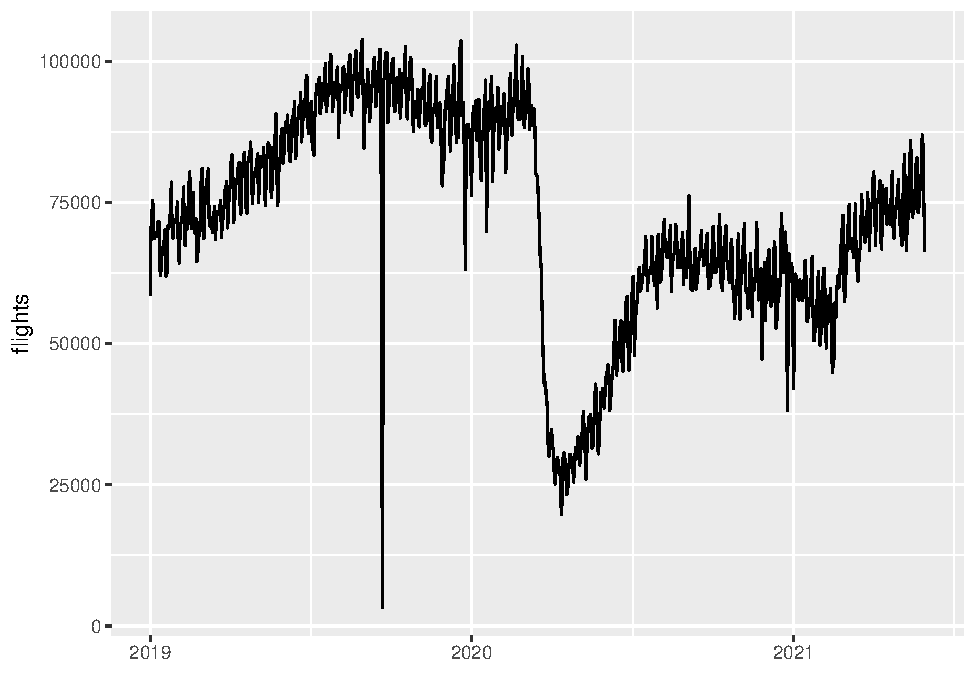
\includegraphics{paper_files/figure-latex/osndaily-1.pdf}
\caption{\label{fig:osndaily}Daily flights tracked by Opensky Network}
\end{figure}

\hypertarget{resultsdiscussion}{%
\section{Results/Discussion}\label{resultsdiscussion}}

1.1

\begin{enumerate}
\def\labelenumi{\alph{enumi})}
\tightlist
\item
  Resilience can be measured as a function of time - the smaller the relationship between time of stress and the time of recovery, more resilient a system is.
\end{enumerate}

1.2 how to use open data to ``see'' resilience?

1.2.1 Gather and prepare data

\begin{Shaded}
\begin{Highlighting}[]
\CommentTok{\#Reading raw data}

\FunctionTok{source}\NormalTok{(}\StringTok{"./R/list\_apt\_files.R"}\NormalTok{)}

\CommentTok{\#Here I will assign only one month {-} "202105". If you want to include a full year, just assign year to "2021" or "2020". It works.}
\NormalTok{year }\OtherTok{\textless{}{-}} \StringTok{"2021"}
\NormalTok{file\_names }\OtherTok{\textless{}{-}} \FunctionTok{list\_apt\_files}\NormalTok{(}\AttributeTok{.year =}\NormalTok{ year)}
\NormalTok{open\_sky }\OtherTok{\textless{}{-}} \FunctionTok{map\_dfr}\NormalTok{(file\_names, read\_csv)}
\end{Highlighting}
\end{Shaded}

\begin{verbatim}
## 
## -- Column specification --------------------------------------------------------
## cols(
##   callsign = col_character(),
##   number = col_character(),
##   icao24 = col_character(),
##   registration = col_character(),
##   typecode = col_character(),
##   origin = col_character(),
##   destination = col_character(),
##   firstseen = col_datetime(format = ""),
##   lastseen = col_datetime(format = ""),
##   day = col_datetime(format = ""),
##   latitude_1 = col_double(),
##   longitude_1 = col_double(),
##   altitude_1 = col_double(),
##   latitude_2 = col_double(),
##   longitude_2 = col_double(),
##   altitude_2 = col_double()
## )
## 
## 
## -- Column specification --------------------------------------------------------
## cols(
##   callsign = col_character(),
##   number = col_character(),
##   icao24 = col_character(),
##   registration = col_character(),
##   typecode = col_character(),
##   origin = col_character(),
##   destination = col_character(),
##   firstseen = col_datetime(format = ""),
##   lastseen = col_datetime(format = ""),
##   day = col_datetime(format = ""),
##   latitude_1 = col_double(),
##   longitude_1 = col_double(),
##   altitude_1 = col_double(),
##   latitude_2 = col_double(),
##   longitude_2 = col_double(),
##   altitude_2 = col_double()
## )
## 
## 
## -- Column specification --------------------------------------------------------
## cols(
##   callsign = col_character(),
##   number = col_character(),
##   icao24 = col_character(),
##   registration = col_character(),
##   typecode = col_character(),
##   origin = col_character(),
##   destination = col_character(),
##   firstseen = col_datetime(format = ""),
##   lastseen = col_datetime(format = ""),
##   day = col_datetime(format = ""),
##   latitude_1 = col_double(),
##   longitude_1 = col_double(),
##   altitude_1 = col_double(),
##   latitude_2 = col_double(),
##   longitude_2 = col_double(),
##   altitude_2 = col_double()
## )
## 
## 
## -- Column specification --------------------------------------------------------
## cols(
##   callsign = col_character(),
##   number = col_character(),
##   icao24 = col_character(),
##   registration = col_character(),
##   typecode = col_character(),
##   origin = col_character(),
##   destination = col_character(),
##   firstseen = col_datetime(format = ""),
##   lastseen = col_datetime(format = ""),
##   day = col_datetime(format = ""),
##   latitude_1 = col_double(),
##   longitude_1 = col_double(),
##   altitude_1 = col_double(),
##   latitude_2 = col_double(),
##   longitude_2 = col_double(),
##   altitude_2 = col_double()
## )
## 
## 
## -- Column specification --------------------------------------------------------
## cols(
##   callsign = col_character(),
##   number = col_character(),
##   icao24 = col_character(),
##   registration = col_character(),
##   typecode = col_character(),
##   origin = col_character(),
##   destination = col_character(),
##   firstseen = col_datetime(format = ""),
##   lastseen = col_datetime(format = ""),
##   day = col_datetime(format = ""),
##   latitude_1 = col_double(),
##   longitude_1 = col_double(),
##   altitude_1 = col_double(),
##   latitude_2 = col_double(),
##   longitude_2 = col_double(),
##   altitude_2 = col_double()
## )
\end{verbatim}

\begin{Shaded}
\begin{Highlighting}[]
\CommentTok{\#Selecting relevant variables}

\NormalTok{fb }\OtherTok{\textless{}{-}}\NormalTok{ open\_sky }\SpecialCharTok{\%\textgreater{}\%} \FunctionTok{transmute}\NormalTok{(}\AttributeTok{ADEP =}\NormalTok{ origin, }\AttributeTok{ADES =}\NormalTok{ destination, }\AttributeTok{TYPE =} \FunctionTok{as.factor}\NormalTok{(typecode), }\AttributeTok{DATE =} \FunctionTok{date}\NormalTok{(day), }\AttributeTok{CALL =}\NormalTok{ callsign}
                             \CommentTok{\#, ACFT\_ID = aircraft\_uid}
\NormalTok{                             )}


\CommentTok{\#Easily "dropping NA\textquotesingle{}s\# {-} this can be further sofisticated}

\NormalTok{fb1 }\OtherTok{\textless{}{-}}\NormalTok{ fb }\SpecialCharTok{\%\textgreater{}\%} \FunctionTok{drop\_na}\NormalTok{()}
\NormalTok{fb1}
\end{Highlighting}
\end{Shaded}

\begin{verbatim}
## # A tibble: 3,338,649 x 5
##    ADEP  ADES  TYPE  DATE       CALL   
##    <chr> <chr> <fct> <date>     <chr>  
##  1 KJFK  LSGG  B788  2021-01-01 ETH726 
##  2 KMIA  KMIA  B763  2021-01-01 LCO1108
##  3 VHHH  71KY  G650  2021-01-01 ABW9515
##  4 OMDM  YSSY  A343  2021-01-01 ASY052 
##  5 KLAX  EDDF  B77L  2021-01-01 CSN461 
##  6 EBLG  EBLG  B744  2021-01-01 ATG6652
##  7 KORD  EHAM  B77L  2021-01-01 CSN5203
##  8 FAOR  OMDB  B738  2021-01-01 KQA304 
##  9 YSSY  OMDB  B77W  2021-01-01 UAE415 
## 10 YSSY  WSSS  A332  2021-01-01 ALK302 
## # ... with 3,338,639 more rows
\end{verbatim}

\begin{Shaded}
\begin{Highlighting}[]
\CommentTok{\#Joining to ADEP}
\NormalTok{fb2 }\OtherTok{\textless{}{-}} \FunctionTok{left\_join}\NormalTok{(fb1, apt\_countries, }\AttributeTok{by =} \FunctionTok{c}\NormalTok{(}\StringTok{"ADEP"} \OtherTok{=} \StringTok{"ICAO"}\NormalTok{)) }\SpecialCharTok{\%\textgreater{}\%} \FunctionTok{mutate}\NormalTok{(}\AttributeTok{ADEP\_CTRY =}\NormalTok{ CTRY, }\AttributeTok{.keep =} \StringTok{"unused"}\NormalTok{, }\AttributeTok{.after =}\NormalTok{ ADEP)}
\CommentTok{\#Joining to ADES}
\NormalTok{fb3 }\OtherTok{\textless{}{-}} \FunctionTok{left\_join}\NormalTok{(fb2, apt\_countries, }\AttributeTok{by =} \FunctionTok{c}\NormalTok{(}\StringTok{"ADES"} \OtherTok{=} \StringTok{"ICAO"}\NormalTok{)) }\SpecialCharTok{\%\textgreater{}\%} \FunctionTok{mutate}\NormalTok{(}\AttributeTok{ADES\_CTRY =}\NormalTok{ CTRY, }\AttributeTok{.keep =} \StringTok{"unused"}\NormalTok{, }\AttributeTok{.after =}\NormalTok{ ADES)}

\CommentTok{\#Check  NA\textquotesingle{}s}
\FunctionTok{colSums}\NormalTok{(}\FunctionTok{is.na}\NormalTok{(fb3))}
\end{Highlighting}
\end{Shaded}

\begin{verbatim}
##      ADEP ADEP_CTRY      ADES ADES_CTRY      TYPE      DATE      CALL 
##         0      1271         0      1446         0         0         0
\end{verbatim}

\begin{Shaded}
\begin{Highlighting}[]
\CommentTok{\# Very few NA\textquotesingle{}s {-} it\textquotesingle{}s safe to drop and factor now}

\NormalTok{fb4 }\OtherTok{\textless{}{-}}\NormalTok{ fb3 }\SpecialCharTok{\%\textgreater{}\%} \FunctionTok{drop\_na}\NormalTok{() }\SpecialCharTok{\%\textgreater{}\%} \FunctionTok{mutate}\NormalTok{(}\AttributeTok{ADEP\_CTRY =} \FunctionTok{as.factor}\NormalTok{(ADEP\_CTRY), }\AttributeTok{ADES\_CTRY =} \FunctionTok{as.factor}\NormalTok{(ADES\_CTRY))}

\CommentTok{\#NOTE: Here we can adjust the European countries that comprises EU region by editing the "eur\_countries" vector:}
\CommentTok{\# Currently in european countries: "GB" "AD" "ES" "AL" "XK" "AT" "BA" "BE" "BG" "IS" "BY" "UA" "CH" "CZ" "SK" "DE" "RU" "DK" "HR" "EE" "FI" "GG" "JE" "IM" "NL" "IE" "FO" "LU" "NO" "PL" "PT" "SE" "LV" "LT" "FR" "GR" "HU" "IT" "LI" "SI" "MT" "MC" "RO" "TR" "MD" "MK" "GI" "RS" "ME" "SM" "GE" "VA"}

\NormalTok{base\_dataset }\OtherTok{\textless{}{-}}\NormalTok{ fb4 }\SpecialCharTok{\%\textgreater{}\%} \FunctionTok{mutate}\NormalTok{(}\AttributeTok{ADEP\_REG =} \FunctionTok{as.factor}\NormalTok{(}\FunctionTok{case\_when}\NormalTok{(ADEP\_CTRY }\SpecialCharTok{==} \StringTok{"US"} \SpecialCharTok{\textasciitilde{}} \StringTok{"US"}\NormalTok{,}
\NormalTok{                                    ADEP\_CTRY }\SpecialCharTok{==} \StringTok{"BR"} \SpecialCharTok{\textasciitilde{}} \StringTok{"BR"}\NormalTok{,}
\NormalTok{                                    ADEP\_CTRY }\SpecialCharTok{\%in\%}\NormalTok{ eur\_countries }\SpecialCharTok{\textasciitilde{}} \StringTok{"EU"}\NormalTok{,}
                                    \ConstantTok{TRUE} \SpecialCharTok{\textasciitilde{}} \StringTok{"Other"}\NormalTok{)), }\AttributeTok{.after =}\NormalTok{ ADEP\_CTRY) }\SpecialCharTok{\%\textgreater{}\%}
                \FunctionTok{mutate}\NormalTok{(}\AttributeTok{ADES\_REG =} \FunctionTok{as.factor}\NormalTok{(}\FunctionTok{case\_when}\NormalTok{(ADES\_CTRY }\SpecialCharTok{==} \StringTok{"US"} \SpecialCharTok{\textasciitilde{}} \StringTok{"US"}\NormalTok{,}
\NormalTok{                                    ADES\_CTRY }\SpecialCharTok{==} \StringTok{"BR"} \SpecialCharTok{\textasciitilde{}} \StringTok{"BR"}\NormalTok{,}
\NormalTok{                                    ADES\_CTRY }\SpecialCharTok{\%in\%}\NormalTok{ eur\_countries }\SpecialCharTok{\textasciitilde{}} \StringTok{"EU"}\NormalTok{,}
                                    \ConstantTok{TRUE} \SpecialCharTok{\textasciitilde{}} \StringTok{"Other"}\NormalTok{)), }\AttributeTok{.after =}\NormalTok{ ADES\_CTRY)}
\FunctionTok{colSums}\NormalTok{(}\FunctionTok{is.na}\NormalTok{(base\_dataset))}
\end{Highlighting}
\end{Shaded}

\begin{verbatim}
##      ADEP ADEP_CTRY  ADEP_REG      ADES ADES_CTRY  ADES_REG      TYPE      DATE 
##         0         0         0         0         0         0         0         0 
##      CALL 
##         0
\end{verbatim}

\begin{Shaded}
\begin{Highlighting}[]
\CommentTok{\# No NA\textquotesingle{}s {-} yaaayy!!}
\FunctionTok{glimpse}\NormalTok{(base\_dataset)}
\end{Highlighting}
\end{Shaded}

\begin{verbatim}
## Rows: 3,336,679
## Columns: 9
## $ ADEP      <chr> "KJFK", "KMIA", "VHHH", "OMDM", "KLAX", "EBLG", "KORD", "FAO~
## $ ADEP_CTRY <fct> US, US, HK, AE, US, BE, US, ZA, AU, AU, TW, NL, TW, US, QA, ~
## $ ADEP_REG  <fct> US, US, Other, Other, US, EU, US, Other, Other, Other, Other~
## $ ADES      <chr> "LSGG", "KMIA", "71KY", "YSSY", "EDDF", "EBLG", "EHAM", "OMD~
## $ ADES_CTRY <fct> CH, US, US, AU, DE, BE, NL, AE, AE, SG, US, PE, CA, AU, QA, ~
## $ ADES_REG  <fct> EU, US, US, Other, EU, EU, EU, Other, Other, Other, US, Othe~
## $ TYPE      <fct> B788, B763, G650, A343, B77L, B744, B77L, B738, B77W, A332, ~
## $ DATE      <date> 2021-01-01, 2021-01-01, 2021-01-01, 2021-01-01, 2021-01-01,~
## $ CALL      <chr> "ETH726", "LCO1108", "ABW9515", "ASY052", "CSN461", "ATG6652~
\end{verbatim}

\begin{Shaded}
\begin{Highlighting}[]
\FunctionTok{summary}\NormalTok{(base\_dataset)}
\end{Highlighting}
\end{Shaded}

\begin{verbatim}
##      ADEP             ADEP_CTRY        ADEP_REG           ADES          
##  Length:3336679     US     :2225791   BR   :  35791   Length:3336679    
##  Class :character   AU     : 127008   EU   : 596507   Class :character  
##  Mode  :character   DE     : 109611   Other: 478590   Mode  :character  
##                     GB     :  84635   US   :2225791                     
##                     FR     :  64874                                     
##                     CA     :  45627                                     
##                     (Other): 679133                                     
##    ADES_CTRY        ADES_REG            TYPE              DATE           
##  US     :2223845   BR   :  35937   B738   : 356779   Min.   :2021-01-01  
##  AU     : 127206   EU   : 597541   A320   : 234165   1st Qu.:2021-02-14  
##  DE     : 109350   Other: 479356   B737   : 205056   Median :2021-03-26  
##  GB     :  84605   US   :2223845   A321   : 135527   Mean   :2021-03-22  
##  FR     :  65219                   A319   : 118359   3rd Qu.:2021-04-29  
##  CA     :  45727                   E75L   : 112965   Max.   :2021-05-30  
##  (Other): 680727                   (Other):2173828                       
##      CALL          
##  Length:3336679    
##  Class :character  
##  Mode  :character  
##                    
##                    
##                    
## 
\end{verbatim}

\begin{Shaded}
\begin{Highlighting}[]
\CommentTok{\#quick peek}
\NormalTok{base\_dataset}
\end{Highlighting}
\end{Shaded}

\begin{verbatim}
## # A tibble: 3,336,679 x 9
##    ADEP  ADEP_CTRY ADEP_REG ADES  ADES_CTRY ADES_REG TYPE  DATE       CALL   
##    <chr> <fct>     <fct>    <chr> <fct>     <fct>    <fct> <date>     <chr>  
##  1 KJFK  US        US       LSGG  CH        EU       B788  2021-01-01 ETH726 
##  2 KMIA  US        US       KMIA  US        US       B763  2021-01-01 LCO1108
##  3 VHHH  HK        Other    71KY  US        US       G650  2021-01-01 ABW9515
##  4 OMDM  AE        Other    YSSY  AU        Other    A343  2021-01-01 ASY052 
##  5 KLAX  US        US       EDDF  DE        EU       B77L  2021-01-01 CSN461 
##  6 EBLG  BE        EU       EBLG  BE        EU       B744  2021-01-01 ATG6652
##  7 KORD  US        US       EHAM  NL        EU       B77L  2021-01-01 CSN5203
##  8 FAOR  ZA        Other    OMDB  AE        Other    B738  2021-01-01 KQA304 
##  9 YSSY  AU        Other    OMDB  AE        Other    B77W  2021-01-01 UAE415 
## 10 YSSY  AU        Other    WSSS  SG        Other    A332  2021-01-01 ALK302 
## # ... with 3,336,669 more rows
\end{verbatim}

\begin{Shaded}
\begin{Highlighting}[]
\CommentTok{\#}
\CommentTok{\#}
\CommentTok{\#}
\CommentTok{\#NOW IT\textquotesingle{}S TIME TO LOOP TO OTHER MONTHS AND BIND THEM ALL!}
\CommentTok{\#}
\CommentTok{\#}
\CommentTok{\#}
\end{Highlighting}
\end{Shaded}

\begin{Shaded}
\begin{Highlighting}[]
\CommentTok{\#quick first look}
\NormalTok{temp1 }\OtherTok{\textless{}{-}}\NormalTok{ base\_dataset }\SpecialCharTok{\%\textgreater{}\%} \FunctionTok{group\_by}\NormalTok{(DATE, ADEP\_REG, ADES\_REG) }\SpecialCharTok{\%\textgreater{}\%} \FunctionTok{summarize}\NormalTok{(}\AttributeTok{FLIGHTS =} \FunctionTok{n}\NormalTok{(), }\AttributeTok{.groups =} \StringTok{"drop"}\NormalTok{) }\SpecialCharTok{\%\textgreater{}\%}
  \FunctionTok{filter}\NormalTok{(ADEP\_REG }\SpecialCharTok{\%in\%} \FunctionTok{c}\NormalTok{(}\StringTok{"BR"}\NormalTok{, }\StringTok{"EU"}\NormalTok{), ADES\_REG  }\SpecialCharTok{\%in\%} \FunctionTok{c}\NormalTok{(}\StringTok{"BR"}\NormalTok{, }\StringTok{"EU"}\NormalTok{)) }\SpecialCharTok{\%\textgreater{}\%}
  \FunctionTok{mutate}\NormalTok{(}\AttributeTok{ROUTE =} \FunctionTok{paste}\NormalTok{(ADEP\_REG, ADES\_REG, }\AttributeTok{sep =} \StringTok{"{-}"}\NormalTok{), }\AttributeTok{.keep =} \StringTok{"unused"}\NormalTok{, }\AttributeTok{.before =} \StringTok{"FLIGHTS"}\NormalTok{) }\SpecialCharTok{\%\textgreater{}\%}
  \FunctionTok{pivot\_wider}\NormalTok{(}\AttributeTok{names\_from =}\NormalTok{ ROUTE, }\AttributeTok{values\_from =}\NormalTok{ FLIGHTS) }
\NormalTok{temp1}
\end{Highlighting}
\end{Shaded}

\begin{verbatim}
## # A tibble: 149 x 5
##    DATE       `BR-BR` `BR-EU` `EU-BR` `EU-EU`
##    <date>       <int>   <int>   <int>   <int>
##  1 2021-01-01     189       8       7    1792
##  2 2021-01-02     265       7      10    3088
##  3 2021-01-03     264      12       6    3721
##  4 2021-01-04     273       6      11    3446
##  5 2021-01-05     320       5      11    3068
##  6 2021-01-06     262      10       7    2930
##  7 2021-01-07     288       8      11    3088
##  8 2021-01-08     266       3       1    3343
##  9 2021-01-09     253       7      11    2695
## 10 2021-01-10     233       7       7    3371
## # ... with 139 more rows
\end{verbatim}

\begin{Shaded}
\begin{Highlighting}[]
\CommentTok{\#First stab at different levels of traffic}

\NormalTok{n }\OtherTok{\textless{}{-}} \FloatTok{0.5}
\NormalTok{temp1 }\SpecialCharTok{\%\textgreater{}\%} \FunctionTok{ggplot}\NormalTok{(}\FunctionTok{aes}\NormalTok{(}\AttributeTok{x =}\NormalTok{ DATE)) }\SpecialCharTok{+}
  \FunctionTok{geom\_point}\NormalTok{(}\FunctionTok{aes}\NormalTok{(}\AttributeTok{y =} \StringTok{\textasciigrave{}}\AttributeTok{EU{-}EU}\StringTok{\textasciigrave{}}\NormalTok{, }\AttributeTok{color =} \StringTok{\textasciigrave{}}\AttributeTok{EU{-}EU}\StringTok{\textasciigrave{}} \SpecialCharTok{\textgreater{}} \FunctionTok{quantile}\NormalTok{(}\StringTok{\textasciigrave{}}\AttributeTok{EU{-}EU}\StringTok{\textasciigrave{}}\NormalTok{[}\FunctionTok{month}\NormalTok{(DATE) }\SpecialCharTok{\%in\%} \DecValTok{1}\SpecialCharTok{:}\DecValTok{2}\NormalTok{], }\AttributeTok{probs =}\NormalTok{ n)), }\AttributeTok{shape =} \DecValTok{4}\NormalTok{) }\SpecialCharTok{+}
  \FunctionTok{geom\_point}\NormalTok{(}\FunctionTok{aes}\NormalTok{(}\AttributeTok{y =} \StringTok{\textasciigrave{}}\AttributeTok{BR{-}BR}\StringTok{\textasciigrave{}}\NormalTok{, }\AttributeTok{color =} \StringTok{\textasciigrave{}}\AttributeTok{BR{-}BR}\StringTok{\textasciigrave{}} \SpecialCharTok{\textgreater{}} \FunctionTok{quantile}\NormalTok{(}\StringTok{\textasciigrave{}}\AttributeTok{BR{-}BR}\StringTok{\textasciigrave{}}\NormalTok{[}\FunctionTok{month}\NormalTok{(DATE) }\SpecialCharTok{\%in\%} \DecValTok{1}\SpecialCharTok{:}\DecValTok{2}\NormalTok{], }\AttributeTok{probs =}\NormalTok{ n)), }\AttributeTok{shape =} \DecValTok{1}\NormalTok{) }\SpecialCharTok{+}
  \FunctionTok{labs}\NormalTok{(}\AttributeTok{y  =} \StringTok{"Flights"}\NormalTok{) }\SpecialCharTok{+} 
  \FunctionTok{theme}\NormalTok{(}\AttributeTok{legend.position =} \StringTok{"bottom"}\NormalTok{)}
\end{Highlighting}
\end{Shaded}

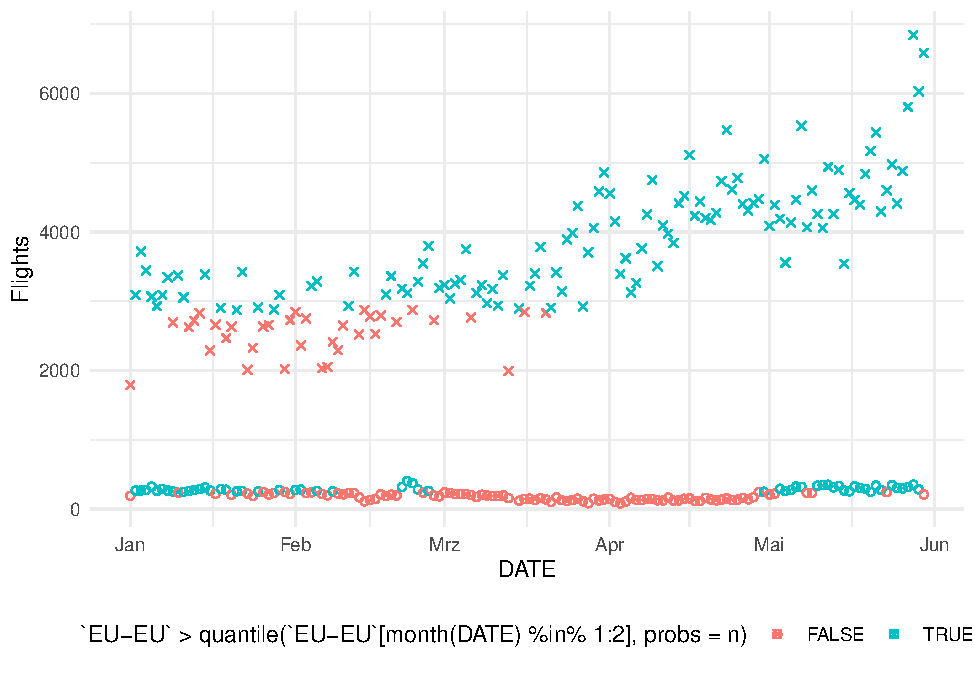
\includegraphics{paper_files/figure-latex/unnamed-chunk-6-1.pdf}

\begin{Shaded}
\begin{Highlighting}[]
\CommentTok{\#Normalized by the median of the last 3 months of the dataset}
\NormalTok{temp2 }\OtherTok{\textless{}{-}}\NormalTok{ temp1 }\SpecialCharTok{\%\textgreater{}\%} \FunctionTok{pivot\_longer}\NormalTok{(}\AttributeTok{cols =} \DecValTok{2}\SpecialCharTok{:}\DecValTok{5}\NormalTok{, }\AttributeTok{names\_to =} \StringTok{"ROUTE"}\NormalTok{, }\AttributeTok{values\_to =} \StringTok{"FLIGHTS"}\NormalTok{) }\SpecialCharTok{\%\textgreater{}\%} \FunctionTok{group\_by}\NormalTok{(ROUTE) }\SpecialCharTok{\%\textgreater{}\%} \FunctionTok{mutate}\NormalTok{(}\AttributeTok{MOVING\_MEDIAN =} \FunctionTok{quantile}\NormalTok{(FLIGHTS[}\FunctionTok{month}\NormalTok{(DATE) }\SpecialCharTok{\%in\%} \FunctionTok{month}\NormalTok{(}\FunctionTok{last}\NormalTok{(DATE))}\SpecialCharTok{{-}}\DecValTok{2}\SpecialCharTok{:}\FunctionTok{month}\NormalTok{(}\FunctionTok{last}\NormalTok{(DATE))], }\AttributeTok{probs =} \FloatTok{0.5}\NormalTok{), }\AttributeTok{NORM\_FLTS =}\NormalTok{ FLIGHTS}\SpecialCharTok{/}\NormalTok{MOVING\_MEDIAN)}
\end{Highlighting}
\end{Shaded}

\begin{verbatim}
## Warning in month(DATE) %in% month(last(DATE)) - 2:month(last(DATE)): Länge des längeren Objektes
##       ist kein Vielfaches der Länge des kürzeren Objektes

## Warning in month(DATE) %in% month(last(DATE)) - 2:month(last(DATE)): Länge des längeren Objektes
##       ist kein Vielfaches der Länge des kürzeren Objektes

## Warning in month(DATE) %in% month(last(DATE)) - 2:month(last(DATE)): Länge des längeren Objektes
##       ist kein Vielfaches der Länge des kürzeren Objektes

## Warning in month(DATE) %in% month(last(DATE)) - 2:month(last(DATE)): Länge des längeren Objektes
##       ist kein Vielfaches der Länge des kürzeren Objektes
\end{verbatim}

\begin{Shaded}
\begin{Highlighting}[]
\NormalTok{temp2}
\end{Highlighting}
\end{Shaded}

\begin{verbatim}
## # A tibble: 596 x 5
## # Groups:   ROUTE [4]
##    DATE       ROUTE FLIGHTS MOVING_MEDIAN NORM_FLTS
##    <date>     <chr>   <int>         <dbl>     <dbl>
##  1 2021-01-01 BR-BR     189          214.     0.881
##  2 2021-01-01 BR-EU       8            7      1.14 
##  3 2021-01-01 EU-BR       7            9      0.778
##  4 2021-01-01 EU-EU    1792         3397      0.528
##  5 2021-01-02 BR-BR     265          214.     1.24 
##  6 2021-01-02 BR-EU       7            7      1    
##  7 2021-01-02 EU-BR      10            9      1.11 
##  8 2021-01-02 EU-EU    3088         3397      0.909
##  9 2021-01-03 BR-BR     264          214.     1.23 
## 10 2021-01-03 BR-EU      12            7      1.71 
## # ... with 586 more rows
\end{verbatim}

\begin{Shaded}
\begin{Highlighting}[]
\NormalTok{temp2 }\SpecialCharTok{\%\textgreater{}\%} \FunctionTok{ggplot}\NormalTok{(}\FunctionTok{aes}\NormalTok{(}\AttributeTok{x =}\NormalTok{ DATE)) }\SpecialCharTok{+}
  \FunctionTok{geom\_line}\NormalTok{(}\FunctionTok{aes}\NormalTok{(}\AttributeTok{y =}\NormalTok{ NORM\_FLTS, }\AttributeTok{color =}\NormalTok{ ROUTE)) }\SpecialCharTok{+}
  \FunctionTok{theme\_minimal}\NormalTok{()}
\end{Highlighting}
\end{Shaded}

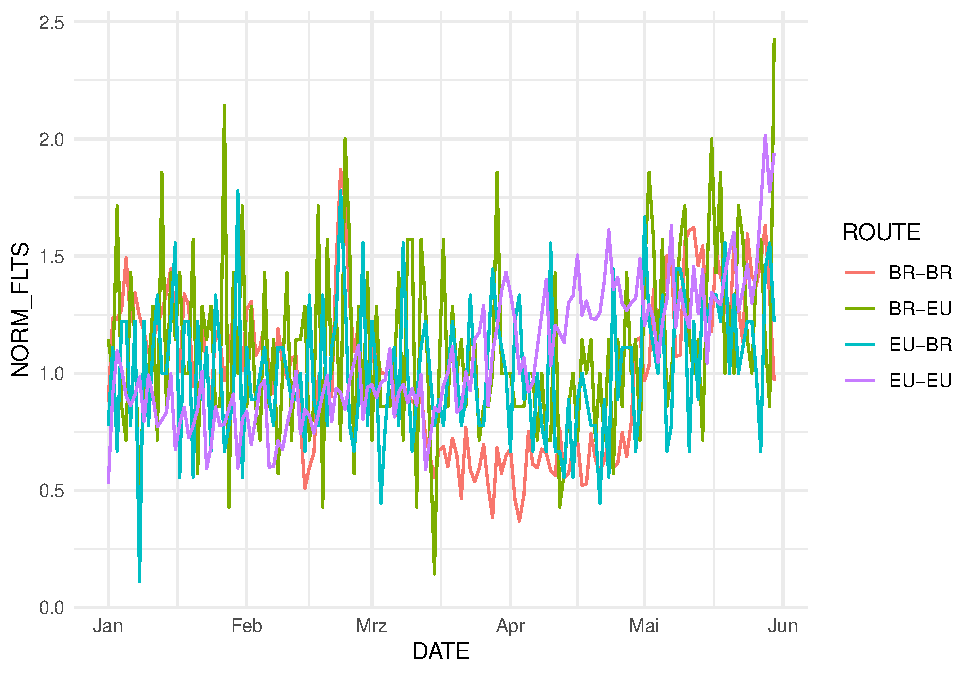
\includegraphics{paper_files/figure-latex/unnamed-chunk-6-2.pdf}

1.2.2

\hypertarget{conclusion}{%
\section{Conclusion}\label{conclusion}}

\hypertarget{acknowledgment}{%
\section*{Acknowledgment}\label{acknowledgment}}
\addcontentsline{toc}{section}{Acknowledgment}

\hypertarget{references}{%
\section*{References}\label{references}}
\addcontentsline{toc}{section}{References}

\hypertarget{refs}{}
\begin{CSLReferences}{1}{0}
\leavevmode\hypertarget{ref-xavier_olive_2021_4893103}{}%
Olive, Xavier, Martin Strohmeier, and Jannis Lübbe. 2021. {``{Crowdsourced air traffic data from The OpenSky Network 2020}.''} Zenodo. \url{https://doi.org/10.5281/zenodo.4893103}.

\leavevmode\hypertarget{ref-strohmeier_crowdsourced_2021}{}%
Strohmeier, Martin, Xavier Olive, Jannis Lübbe, Matthias Schäfer, and Vincent Lenders. 2021. {``Crowdsourced Air Traffic Data from {OpenSky Network} 2019-2020.''} \emph{Earth Systems Science Data} 13: 357--66. \url{https://doi.org/10.5194/essd-13-357-2021}.

\end{CSLReferences}

\end{document}

